\chapter{Présentation de l'organisme d'acceuil (L'\acs{ARCOP})}
\clearpage
\section{Historique et missions de l’\acs{ARCOP}}

\subsection{Historique}
En vue de l’instauration d’un État de droit prospère, le gouvernement togolais a entrepris de profondes réformes institutionnelles. Ainsi, pour se conformer aux dispositions régionales, il a été mis en place l’Autorité de régulation de la commande publique (\ac{ARCOP}), une autorité administrative indépendante investie de plusieurs missions selon les dispositions du décret n° 2009-296/PR du 30 décembre 2009, modifié par le décret n° 2011-182/PR du 28 décembre 2011 portant missions, attributions, organisation et fonctionnement de l’Autorité de Régulation de la Commande Publique.

L’Autorité de régulation de la commande publique est située sur le boulevard GNASSINGBE Eyadema. Elle est logée aux 6ème et 7ème étages de l’immeuble SANLAM, près du siège de Yas-TOGO.

\begin{itemize}
    \item \textbf{Adresse :} B.P. 12 484 Lomé-Togo
    \item \textbf{Téléphone :} (00228) 22 23 06 80 / 22 23 06 81
    \item \textbf{E-mail :} \href{arcoptogo@arcop.tg}{arcoptogo@arcop.tg}
    \item \textbf{Site web :} \href{https://arcop.tg}{https://arcop.tg}
    \item \textbf{N° vert :} 80 00 88 88
\end{itemize}

\subsection{Missions de l’\acs{ARCOP}}
Selon l’article n° 3 du décret n° 2022-063/PR, \og l’Autorité de régulation de la commande publique assure la régulation du système de gestion de la commande publique \fg.

À ce titre, elle :
\begin{itemize}
    \item Émet des avis, propositions ou recommandations dans le cadre de la définition des politiques et de l'assistance à l'élaboration de la réglementation de la commande publique ;
    \item Assure la sensibilisation et l'information des acteurs de la commande publique ;
    \item Élabore des stratégies de professionnalisation et de renforcement des capacités ;
    \item Assure l’évaluation des performances du système de passation et d’exécution ;
    \item Diligente des enquêtes sur les irrégularités et violations ;
    \item Initie des procédures d'audits de conformité et financiers ;
    \item Procède au règlement non juridictionnel des litiges et sanctionne les irrégularités constatées.
\end{itemize}

\section{Les organes de l’\acs{ARCOP}}
Conformément aux dispositions du décret n° 2009-296/PR modifié, l’\ac{ARCOP} est composée de trois organes :
\begin{itemize}
    \item Le Conseil de régulation (CR) ;
    \item Le Comité de règlement des différends (CRD) ;
    \item La Direction générale (DG).
\end{itemize}

\subsection{Le Conseil de régulation (CR)}
L’article n° 11 du décret n° 2022-063/PR stipule que le conseil de régulation est un organe tripartite composé de neuf membres représentant l’administration publique, le secteur privé et la société civile.

\subsection{Le Comité de règlement des différends (CRD)}
L’article n° 22 du décret n° 2022-063/PR stipule que le comité de règlement des différends est chargé de :
\begin{itemize}
    \item Examiner les recours relatifs à la passation des contrats de la commande publique ;
    \item Statuer sur les irrégularités ou violations constatées ;
    \item Régler les différends entre entités administratives impliquées dans la commande publique.
\end{itemize}

\subsection{La Direction générale}
L’article n° 29 du décret n° 2022-063/PR stipule que la direction générale est l'organe exécutif de l’\ac{ARCOP}, chargée de l’application des politiques générales et de la mise en œuvre des décisions du conseil de régulation.

Elle est structurée en six directions :
\begin{itemize}
    \item \textbf{Direction des services administratifs et financiers (DSAF)} : gestion des ressources humaines et financières ;
    \item \textbf{Direction de la réglementation et des affaires juridiques (DRAJ)} : suivi et mise en application des réglementations ;
    \item \textbf{Direction de la formation et des appuis techniques (DFAT)} : renforcement des capacités des acteurs ;
    \item \textbf{Direction des statistiques, documentation et suivi-évaluation (DSD-SE)} : centralisation des données et évaluation des performances ;
    \item \textbf{Direction des investigations et enquêtes (DIE)} : enquêtes sur les irrégularités et lutte contre la corruption ;
    \item \textbf{Direction de la communication et des relations publiques (DCRP)} : gestion de la communication interne et externe.
\end{itemize}

\subsection{Organisation administrative de la Direction générale}

Comme illustré dans la figure \ref{fig:organigramme-arcop}, la Direction générale de l'\ac{ARCOP} est structurée en six directions, chacune chargée d'un aspect spécifique des missions de régulation de la commande publique.


\begin{figure}[H]
    \centering
    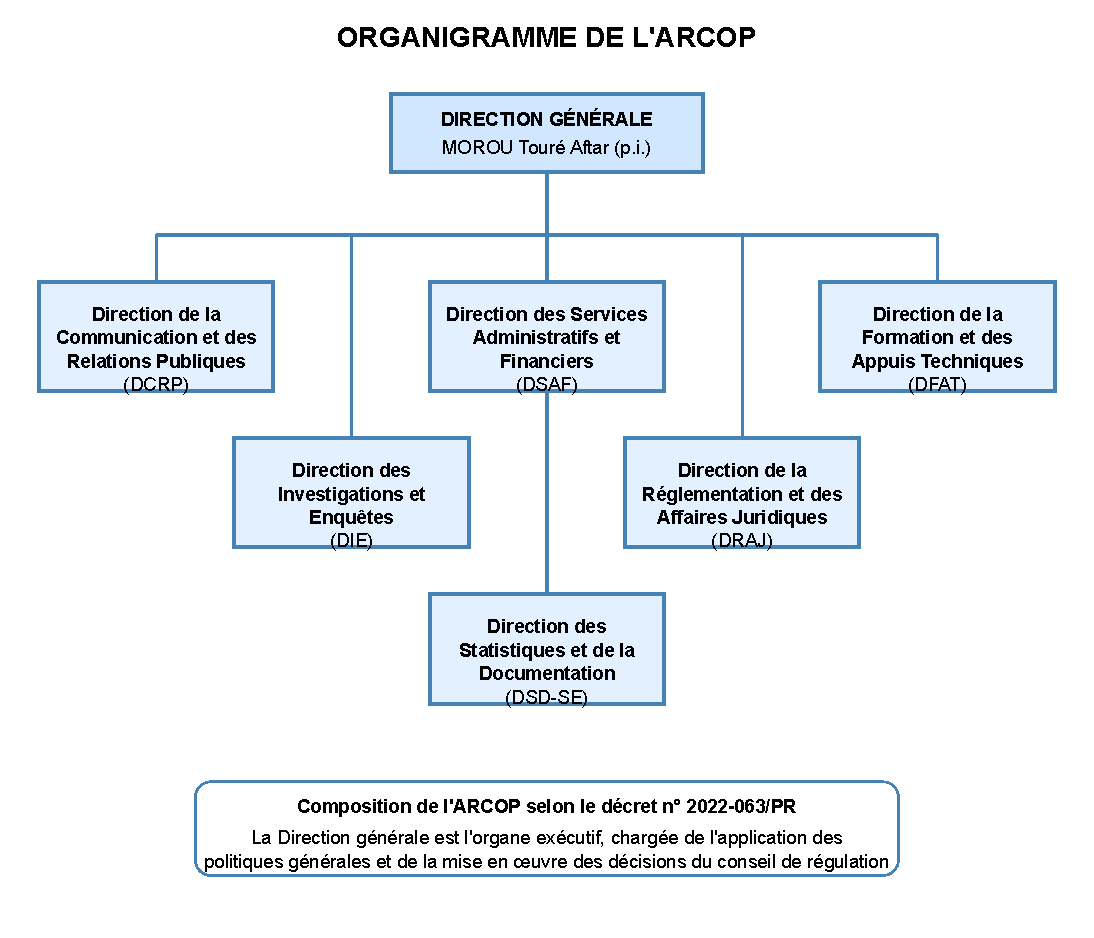
\includegraphics[width=\textwidth]{images/diagrammes/autres/organigramme-arcop.pdf}
    \caption{Organigramme de la Direction générale de l'\ac{ARCOP}}
    \label{fig:organigramme-arcop}
\end{figure}

La Direction générale de l’\ac{ARCOP} exerce une surveillance active sur les processus d'achat public afin de garantir l'intégrité, la transparence et l'efficacité des dépenses publiques, contribuant ainsi au développement économique et social du pays.



\clearpage